%%%%%%%%%%%%%%%%%%%%%%%%%%%%%%%%%%%%%%%%%
% Wenneker Article
% LaTeX Template
% Version 2.0 (28/2/17)
%
% This template was downloaded from:
% http://www.LaTeXTemplates.com
%
% Authors:
% Vel (vel@LaTeXTemplates.com)
% Frits Wenneker
%
% License:
% CC BY-NC-SA 3.0 (http://creativecommons.org/licenses/by-nc-sa/3.0/)
%
%%%%%%%%%%%%%%%%%%%%%%%%%%%%%%%%%%%%%%%%%

%----------------------------------------------------------------------------------------
%	PACKAGES AND OTHER DOCUMENT CONFIGURATIONS
%----------------------------------------------------------------------------------------

\documentclass[10pt, a4paper, twocolumn]{article} % 10pt font size (11 and 12 also possible), A4 paper (letterpaper for US letter) and two column layout (remove for one column)
\usepackage{placeins}
\usepackage{multirow}
\usepackage{amsmath}
\newcommand{\comment}[1]{}
%%%%%%%%%%%%%%%%%%%%%%%%%%%%%%%%%%%%%%%%%
% Wenneker Article
% Structure Specification File
% Version 1.0 (28/2/17)
%
% This file originates from:
% http://www.LaTeXTemplates.com
%
% Authors:
% Frits Wenneker
% Vel (vel@LaTeXTemplates.com)
%
% License:
% CC BY-NC-SA 3.0 (http://creativecommons.org/licenses/by-nc-sa/3.0/)
%
%%%%%%%%%%%%%%%%%%%%%%%%%%%%%%%%%%%%%%%%%

%----------------------------------------------------------------------------------------
%	PACKAGES AND OTHER DOCUMENT CONFIGURATIONS
%----------------------------------------------------------------------------------------

\usepackage[english]{babel} % English language hyphenation

\usepackage{microtype} % Better typography

\usepackage{amsmath,amsfonts,amsthm} % Math packages for equations

\usepackage[svgnames]{xcolor} % Enabling colors by their 'svgnames'

\usepackage[hang, small, labelfont=bf, up, textfont=it]{caption} % Custom captions under/above tables and figures

\usepackage{booktabs} % Horizontal rules in tables

\usepackage{lastpage} % Used to determine the number of pages in the document (for "Page X of Total")

\usepackage{graphicx} % Required for adding images

\usepackage{enumitem} % Required for customising lists
\setlist{noitemsep} % Remove spacing between bullet/numbered list elements

\usepackage{sectsty} % Enables custom section titles
\allsectionsfont{\usefont{OT1}{phv}{b}{n}} % Change the font of all section commands (Helvetica)

%----------------------------------------------------------------------------------------
%	MARGINS AND SPACING
%----------------------------------------------------------------------------------------

\usepackage{geometry} % Required for adjusting page dimensions

\geometry{
	top=1cm, % Top margin
	bottom=1.5cm, % Bottom margin
	left=2cm, % Left margin
	right=2cm, % Right margin
	includehead, % Include space for a header
	includefoot, % Include space for a footer
	%showframe, % Uncomment to show how the type block is set on the page
}

\setlength{\columnsep}{7mm} % Column separation width

%----------------------------------------------------------------------------------------
%	FONTS
%----------------------------------------------------------------------------------------

\usepackage[T1]{fontenc} % Output font encoding for international characters
\usepackage[utf8]{inputenc} % Required for inputting international characters

\usepackage{XCharter} % Use the XCharter font

%----------------------------------------------------------------------------------------
%	HEADERS AND FOOTERS
%----------------------------------------------------------------------------------------

\usepackage{fancyhdr} % Needed to define custom headers/footers
\pagestyle{fancy} % Enables the custom headers/footers

\renewcommand{\headrulewidth}{0.0pt} % No header rule
\renewcommand{\footrulewidth}{0.4pt} % Thin footer rule

\renewcommand{\sectionmark}[1]{\markboth{#1}{}} % Removes the section number from the header when \leftmark is used

%\nouppercase\leftmark % Add this to one of the lines below if you want a section title in the header/footer

% Headers
\lhead{} % Left header
\chead{\textit{\thetitle}} % Center header - currently printing the article title
\rhead{} % Right header

% Footers
\lfoot{} % Left footer
\cfoot{} % Center footer
\rfoot{\footnotesize Page \thepage\ of \pageref{LastPage}} % Right footer, "Page 1 of 2"

\fancypagestyle{firstpage}{ % Page style for the first page with the title
	\fancyhf{}
	\renewcommand{\footrulewidth}{0pt} % Suppress footer rule
}

%----------------------------------------------------------------------------------------
%	TITLE SECTION
%----------------------------------------------------------------------------------------

\newcommand{\authorstyle}[1]{{\large\usefont{OT1}{phv}{b}{n}\color{DarkRed}#1}} % Authors style (Helvetica)

\newcommand{\institution}[1]{{\footnotesize\usefont{OT1}{phv}{m}{sl}\color{Black}#1}} % Institutions style (Helvetica)

\usepackage{titling} % Allows custom title configuration

\newcommand{\HorRule}{\color{DarkGoldenrod}\rule{\linewidth}{1pt}} % Defines the gold horizontal rule around the title

\pretitle{
	\vspace{-30pt} % Move the entire title section up
	\HorRule\vspace{10pt} % Horizontal rule before the title
	\fontsize{32}{36}\usefont{OT1}{phv}{b}{n}\selectfont % Helvetica
	\color{DarkRed} % Text colour for the title and author(s)
}

\posttitle{\par\vskip 15pt} % Whitespace under the title

\preauthor{} % Anything that will appear before \author is printed

\postauthor{ % Anything that will appear after \author is printed
	\vspace{10pt} % Space before the rule
	\par\HorRule % Horizontal rule after the title
	\vspace{20pt} % Space after the title section
}

%----------------------------------------------------------------------------------------
%	ABSTRACT
%----------------------------------------------------------------------------------------

\usepackage{lettrine} % Package to accentuate the first letter of the text (lettrine)
\usepackage{fix-cm}	% Fixes the height of the lettrine

\newcommand{\initial}[1]{ % Defines the command and style for the lettrine
	\lettrine[lines=3,findent=4pt,nindent=0pt]{% Lettrine takes up 3 lines, the text to the right of it is indented 4pt and further indenting of lines 2+ is stopped
		\color{DarkGoldenrod}% Lettrine colour
		{#1}% The letter
	}{}%
}

\usepackage{xstring} % Required for string manipulation

\newcommand{\lettrineabstract}[1]{
	\StrLeft{#1}{1}[\firstletter] % Capture the first letter of the abstract for the lettrine
	\initial{\firstletter}\textbf{\StrGobbleLeft{#1}{1}} % Print the abstract with the first letter as a lettrine and the rest in bold
}

%----------------------------------------------------------------------------------------
%	BIBLIOGRAPHY
%----------------------------------------------------------------------------------------

\usepackage[backend=bibtex,style=authoryear,natbib=true]{biblatex} % Use the bibtex backend with the authoryear citation style (which resembles APA)

\addbibresource{example.bib} % The filename of the bibliography

\usepackage[autostyle=true]{csquotes} % Required to generate language-dependent quotes in the bibliography
 % Specifies the document structure and loads requires packages

%----------------------------------------------------------------------------------------
%	ARTICLE INFORMATION
%----------------------------------------------------------------------------------------

\title{MLPR Exam Project: \\Gender Detection} % The article title

\author{
	\authorstyle{Mattia Rosso [s294711]} % Author
	%\newline\newline % Space before institutions
	%\textsuperscript{1}\institution{Universidad Nacional Autónoma de México, Mexico City, Mexico}\\ % Institution 1
	%\textsuperscript{2}\institution{University of Texas at Austin, Texas, United States of America}\\ % Institution 2
	%\textsuperscript{3}\institution{\texttt{LaTeXTemplates.com}} % Institution 3
}

% Example of a one line author/institution relationship
%\author{\newauthor{John Marston} \newinstitution{Universidad Nacional Autónoma de México, Mexico City, Mexico}}

\date{\today} % Add a date here if you would like one to appear underneath the title block, use \today for the current date, leave empty for no date

%----------------------------------------------------------------------------------------

\begin{document}
\maketitle % Print the title
\thispagestyle{firstpage} % Apply the page style for the first page (no headers and footers)

%----------------------------------------------------------------------------------------
%	ABSTRACT
%----------------------------------------------------------------------------------------

\lettrineabstract{This project is inteded to show a binary classification 
task on a datased made of 12 continuous observations coming from speking embeddings. 
A speaker embedding represents a smal-dimensional, fixed size representation of an utterance.
Features can be seen as points in the m-dimensional embedding space (and the embeddings
have already been computed). This is a task where classes are balanced both in training and
evaluation set}

%----------------------------------------------------------------------------------------
%	ARTICLE CONTENTS
%----------------------------------------------------------------------------------------

\section{Dataset analysis}
\subsection{Training and evaluation sets}
The training set contains:
\begin{itemize}
	\item Training Set: 3000 samples belonging to Male class (Label = 0) and
						3000 samples belonging to Female class (Label = 1).
	\item Evaluation Set: 2000 samples belonging to Male class (Label = 0) and
						  2000 samples belonging to Female class (Label = 1).
\end{itemize}

\subsection{Training set features analysis}
\subsection{Features Statistics}
All the features are contiguous and their main statics can be
showed through a boxplot in figure \ref{boxplot}. 

\subsection{Z-normalization}
A useful operation that can be applied in order to avoid to deal with numerical 
issues and to make data more uniform is to apply Z-normalization as a preprocessing step:\\
\begin{center}
	\begin{math}
		z_{i,j} = \frac{x_{i,j} - \mu_{j}}{\sigma_{j}} \forall x_{i} \in D 
	\end{math}
\end{center}
Where $z_{i,j}$ is the Z-normalized value correspongin to the feature $j$
of sample $i$ while $\mu_{j}$ and $\sigma_{j}$ are, respectively,
the mean and the variance computed over all values for feature $j$.
\comment{
\FloatBarrier
	\begin{table}
		\caption{Features Statistics}
		\centering
		\begin{tabular}{ |l|l|l|l|l| }
			\hline
			\multicolumn{5}{ |c| }{Statistics} \\
			\hline
			Feature & Min & Max & Mean & StdDev \\ \hline
			\multirow{2}{*}{0}
			 & 0 & 0 & 0 & 0 \\
			 & 0 & 0 & 0 & 0  \\ \hline
			\multirow{2}{*}{1}
			 & 0 & 0 & 0 & 0  \\
			 & 0 & 0 & 0 & 0  \\ \hline
			\multirow{2}{*}{2}
			& 0 & 0 & 0 & 0  \\
			& 0 & 0 & 0 & 0  \\ \hline
		\end{tabular}
	\end{table}
\FloatBarrier
}
\begin{figure}[ht!]
	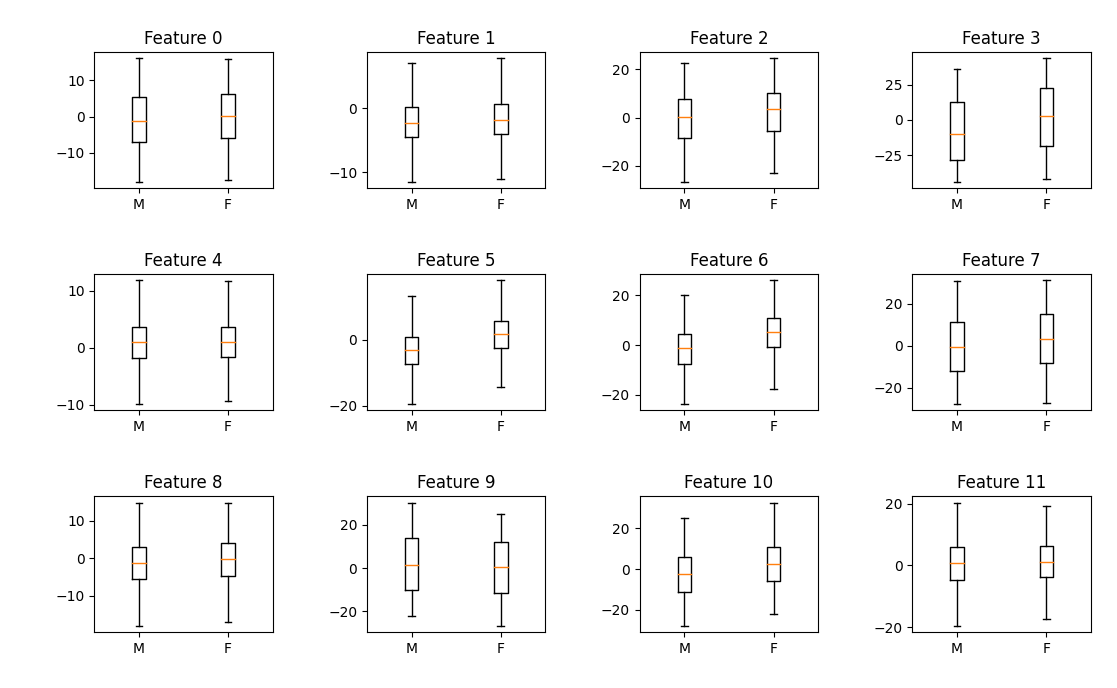
\includegraphics[width=\linewidth]{./Pictures/FeaturesAnalysis/boxplot.png}
	\caption{Features boxplot}
	\label{boxplot} 
\end{figure}

\subsection{Features distribution}
By plotting historams for each feature, separated for male and female, it is possible to show
how much each feature follows a gaussian distribution in order to understend whether a pre processing
like gaussianization can be useful to go on with our classification task
\begin{figure}[ht!]
	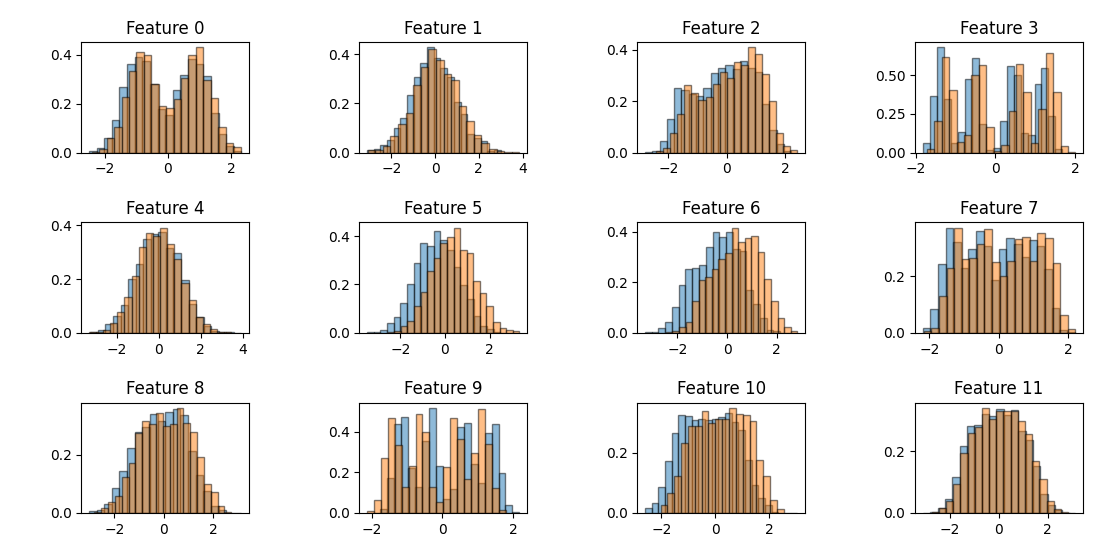
\includegraphics[width=\linewidth]{./Pictures/FeaturesAnalysis/hist_znorm.png}
	\caption{Z-normalized features distribution}
	\label{hist_znorm} 
\end{figure}

We can notice from figure \ref{hist_znorm} that almost all the features are already 
well-distributed except for features 3, 7, 9. We can apply an additional pre-processing step in
order to make all the features following a gaussian distribution.

\subsubsection{Gaussianization}
Gaussianization is a pre processing step that maps each fature to values whose empirical cumulative
distribution is well approximated by a Gaussian cumulative distribution function. For each
feature $x$ that we want to gaussianize we firstly compute the rank over the dataset:\\
\begin{center}
	\begin{math}
		r(x) = \frac{\sum_{i=1}^{N}\mathbb{I}[x_{i} < x] + 1}{N + 2}
	\end{math}
\end{center}
where $\mathbb{I}$ is the indicator function ($1$ when the condition inside $[ ]$ is true, $0$ 
otherwise). Actually, we are counting how many samples in the dataset $D$ have a greater value
with respect to the feature we are computing the rank on. \\
The next step is to compute the transformed feature as $y = \Phi^{-1}(r(x))$ where $\Phi$ is
the inverse of the cumulative distribution function. 

\begin{figure}[ht!]
	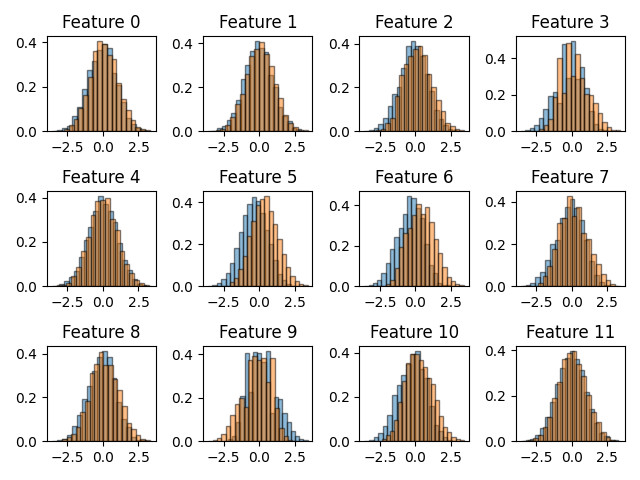
\includegraphics[width=\linewidth]{./Pictures/FeaturesAnalysis/hist_gau.png}
	\caption{Gaussianized features distribution}
	\label{hist_gau} 
\end{figure}

\subsection{Features correlation}
We can show how much features are correlated by using a heatmap plot showing a darker
color inside cells $[i, j]$ for which it exists an high correlation among feaure $i$ and 
feature $j$. We are going to use the Pearson correlation coefficient to compute the
correlation among feature $X$ and feature $Y$:
\begin{center}
	\begin{math}
		|\frac{Cov(X, Y)}{\sqrt{Var(X)}\sqrt{Var(Y)}}|
	\end{math}
\end{center}
\begin{figure}[ht!]
	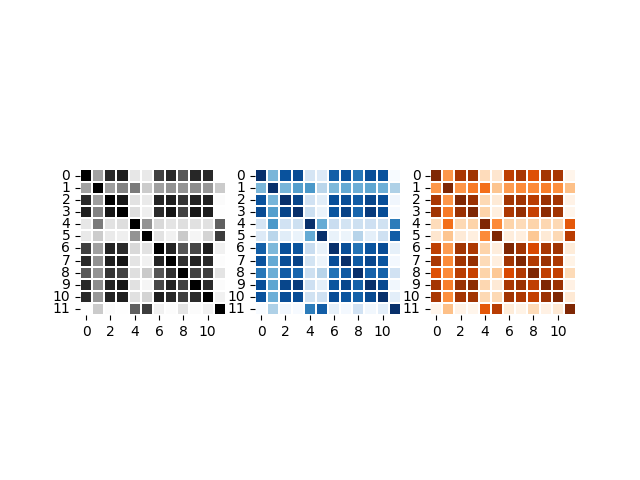
\includegraphics[width=\linewidth]{./Pictures/FeaturesAnalysis/heatmap_znormgau.png}
	\caption{Z-normalized+Gaussianized features correlation: grey the whole dataset, orange F class, 
	blue M class}
	\label{heatmap} 
\end{figure}

Correlation is quite high among most of the features, we can understand that applying PCA
would be meaningful for values of $m$ not below $10$ or $9$ at most. For smaller values of $m$
we would lose important information coming from high-correlated features. 

\section{Dimensionality reduction}
Before proceeding with the classification task i would spend some words on the possible 
dimensioanlity reduction rechniques that can be applied: PCA, LDA.
\subsection{PCA}
As already anticipated, given the heatmap in figure \ref{heatmap} we can observe that PCA
with reasonable values of $m$ can be applied. PCA is a dimensionality reduction technique
that, given a centered dataset $X = {x_{1}, ..., x_{k}}$, it aims to find the subspace of 
$\mathbb{R}^{n}$ that allows to preserve most of the information (the directions with the
highest variance).\\Starting from the sample covariance matrix
\begin{center}
	\begin{math}
		C = \frac{1}{K} \sum_{i}^{}(x_{i} - \bar{x})(x_{i}-\bar{x})^T
	\end{math}
\end{center}
we compute the eigen-decomposition of $C = U\Sigma U^T$ and project the data in the subspace
spanned by the $m$ columns of $U$ corresponding to the $m$ highest eigenvalues:
\begin{center}
	\begin{math}
		y_{i} = P^T(x_{i}-\bar{x})
	\end{math}
\end{center}
In order to select the optimal $m$ we can use a cross-validation approach by inspecting how much
of the total variance of data we are able to retain by using that value of $m$. We exploit the fact
that each eigenvalue correspond to the variance along the corresponding axis and the
eigenvalues are the elements of the diagonal of the matrix $\Sigma$. We selecte $m$ as:
\begin{center}
	\begin{math}
		\min_m\;s.t \frac{\sum_{i}^{m}\sigma_{i}}{\sum_{i}^{n}\sigma_{i}} >= t,\;t \ge 95\%
	\end{math}
\end{center}
\begin{figure}[ht!]
	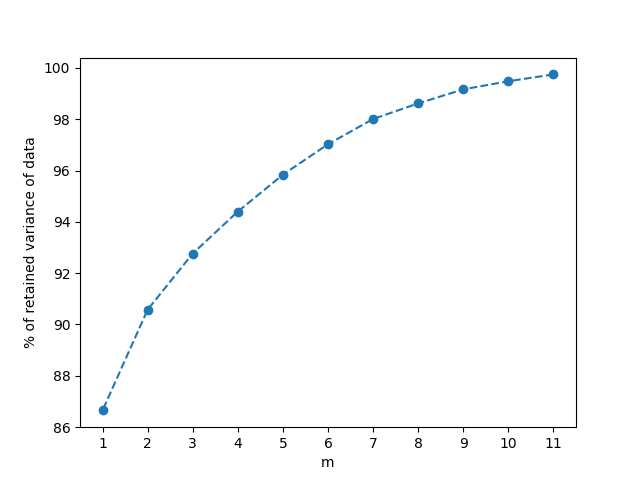
\includegraphics[width=\linewidth]{./Pictures/FeaturesAnalysis/pca.png}
	\caption{3-fold cross validation for PCA impact evaluation}
	\label{pca} 
\end{figure}
We can clearly understand from figure \ref{pca} that values of $m < 9$ would rapidly
decrease the amout of retained variance. We will see better later on how this would 
badly impact the performance of the classifiers

\subsection{LDA}
PCA technique is unsupervised so we have no guarantee of obtainig discriminant directions.
Despite the fact that LDA allows to find at most $C - 1$, where $C$ is the number of classes,
directions, so it makes no sense to apply it as a dimensionality reduction technique, it can
be used as a linear classifier and we can understand it by its definition; LDA mazimizes the
between-class variability over the within-class variability ratio for the transformed samples:
\begin{center}
	\begin{math}
		\mathcal{L}(w) = \frac{s_{B}}{s_{W}} = \max_w \frac{w^TS_{B}w}{w^TS_{W}w}
	\end{math}
\end{center}
It can be proved that optimal solution correspond to the eigenvector of $S_{W}^-1S_{B}$ 
corresponding to the largest eigenvalue. Once that we have estimated $w$ we can project
the test samples over $w$ and assign the class label looking at the score obtained:\\
\begin{center}
	\begin{math}
		f(x)=\left\{
		\begin{array}{ll}
			1, & \mbox{if $x<0$}.\\
			0, & \mbox{otherwise}.
		\end{array}
		\right.
	\end{math}
\end{center}
It will be showed later the result of the classifier
\section{Classification models analysis}
\susection{Premises}
In the next paragraphs we are going to compare different classification models. 
We will employ a k-fold cross validation technique (with $k=3$) for model evaluation and the
best models will be chosen to train the entire training set for performing a final comparison.
We will consider three types of applications:
\begin{center}
	$(\tilde{\pi}, C_{fp}, C_{fn}) = (0.1, 1, 1)$\\
	$(\tilde{\pi}, C_{fp}, C_{fn}) = (0.5, 1, 1)$\\
	$(\tilde{\pi}, C_{fp}, C_{fn}) = (0.9, 1, 1)$\\
\end{center}
and the target application will be 
\begin{center}
	$(\tilde{\pi}, C_{fp}, C_{fn}) = (0.5, 1, 1)$
\end{center}
We are interested
in selecting the most promising approach and we will infact perform measures in term of minimum
detection cost:
\begin{center}
	\begin{math}
		DCF = \frac{DCF_{u}(\pi_{T}, C_{fn}, C_{fp})}{min(\pi_{T},C_{fn}, (1-\pi_{T}C_{fp}))} = 
			\frac{\pi_{T}C_{fn}P_{fn} + (1-\pi_{T})C_{fp}P_{fp}}{min(\pi_{T},C_{fn}, (1-\pi_{T}C_{fp}))}
	\end{math}
\end{center}
and for $minDCF$ computation we will look for:
\begin{center}
	\begin{math}
		t' = -log(\frac{\tilde{\pi}}{1-\tilde{\pi}})
	\end{math}
\end{center}
that allows us to obtain the lowest possible $DCF$ (as if knew in advance this optimal threshold)
\subsection{Gaussian models}
The first class of models we are going to analyze are the generative gaussian models. Model assumption are that,
given the dataset $X$ we assume that the sample $x_{t}$ is a realization of the R.V. $X_{t}$. A simple
model consists in assuming that our data, given the class, can be described by a Gaussian distribution:
\begin{center}
	\begin{math}
		(X_{t}|C_{t}=c) \sim (X|C=c) \sim \mathcal{N} (x_{t}|\mu_{c},\Sigma_{c})
	\end{math}
\end{center}
%------------------------------------------------

\subsection{Subsection}

Nam ante risus, tempor nec lacus ac, congue pretium dui. Donec a nisl est. Integer accumsan mauris eu ex venenatis mollis. Aliquam sit amet ipsum laoreet, mollis sem sit amet, pellentesque quam. Aenean auctor diam eget erat venenatis laoreet. In ipsum felis, tristique eu efficitur at, maximus ac urna. Aenean pulvinar eu lorem eget suscipit. Aliquam et lorem erat. Nam fringilla ante risus, eget convallis nunc pellentesque non. Donec ipsum nisl, consectetur in magna eu, hendrerit pulvinar orci. Mauris porta convallis neque, non viverra urna pulvinar ac. Cras non condimentum lectus. Aliquam odio leo, aliquet vitae tellus nec, imperdiet lacinia turpis. Nam ac lectus imperdiet, luctus nibh a, feugiat urna.

\begin{itemize}
	\item First item in a list 
	\item Second item in a list 
	\item Third item in a list
\end{itemize}

Nunc egestas quis leo sed efficitur. Donec placerat, dui vel bibendum bibendum, tortor ligula auctor elit, aliquet pulvinar leo ante nec tellus. Praesent at vulputate libero, sit amet elementum magna. Pellentesque sodales odio eu ex interdum molestie. Suspendisse lacinia, augue quis interdum posuere, dolor ipsum euismod turpis, sed viverra nibh velit eget dolor. Curabitur consectetur tempus lacus, sit amet luctus mauris interdum vel. Curabitur vehicula convallis felis, eget mattis justo rhoncus eget. Pellentesque et semper lectus.

\begin{description}
	\item[First] This is the first item
	\item[Last] This is the last item
\end{description}

Donec nec nibh sagittis, finibus mauris quis, laoreet augue. Maecenas aliquam sem nunc, vel semper urna hendrerit nec. Pellentesque habitant morbi tristique senectus et netus et malesuada fames ac turpis egestas. Maecenas pellentesque dolor lacus, sit amet pretium felis vestibulum finibus. Duis tincidunt sapien faucibus nisi vehicula tincidunt. Donec euismod suscipit ligula a tempor. Aenean a nulla sit amet magna ullamcorper condimentum. Fusce eu velit vitae libero varius condimentum at sed dui.

%------------------------------------------------

\subsection{Subsection}

In hac habitasse platea dictumst. Etiam ac tortor fermentum, ultrices libero gravida, blandit metus. Vivamus sed convallis felis. Cras vel tortor sollicitudin, vestibulum nisi at, pretium justo. Curabitur placerat elit nunc, sed luctus ipsum auctor a. Nulla feugiat quam venenatis nulla imperdiet vulputate non faucibus lorem. Curabitur mollis diam non leo ullamcorper lacinia.

Morbi iaculis posuere arcu, ut scelerisque sem. Class aptent taciti sociosqu ad litora torquent per conubia nostra, per inceptos himenaeos. Mauris placerat urna id enim aliquet, non consequat leo imperdiet. Phasellus at nibh ut tortor hendrerit accumsan. Phasellus sollicitudin luctus sapien, feugiat facilisis risus consectetur eleifend. In quis luctus turpis. Nulla sed tellus libero. Pellentesque metus tortor, convallis at tellus quis, accumsan faucibus nulla. Fusce auctor eleifend volutpat. Maecenas vel faucibus enim. Donec venenatis congue congue. Integer sit amet quam ac est aliquam aliquet. Ut commodo justo sit amet convallis scelerisque.

\begin{enumerate}
	\item First numbered item in a list
	\item Second numbered item in a list
	\item Third numbered item in a list
\end{enumerate}

Aliquam elementum nulla at arcu finibus aliquet. Praesent congue ultrices nisl pretium posuere. Nunc vel nulla hendrerit, ultrices justo ut, ultrices sapien. Duis ut arcu at nunc pellentesque consectetur. Vestibulum eget nisl porta, ultricies orci eget, efficitur tellus. Maecenas rhoncus purus vel mauris tincidunt, et euismod nibh viverra. Mauris ultrices tellus quis ante lobortis gravida. Duis vulputate viverra erat, eu sollicitudin dui. Proin a iaculis massa. Nam at turpis in sem malesuada rhoncus. Aenean tempor risus dui, et ultrices nulla rutrum ut. Nam commodo fermentum purus, eget mattis odio fringilla at. Etiam congue et ipsum sed feugiat. Morbi euismod ut purus et tempus. Etiam est ligula, aliquam eget porttitor ut, auctor in risus. Curabitur at urna id dui lobortis pellentesque.


%------------------------------------------------

\section{Section}

\begin{figure}[htpb!]
	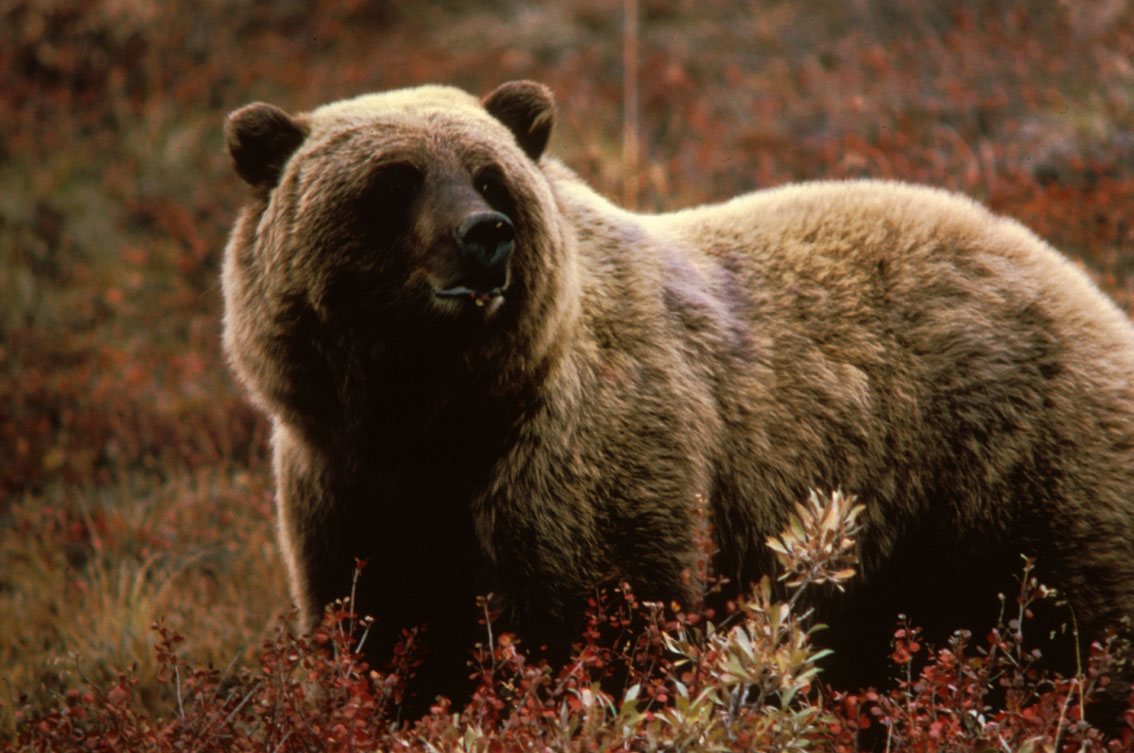
\includegraphics[width=\linewidth]{bear.jpg} % Figure image
	\caption{A majestic grizzly bear} % Figure caption
	\label{bear} % Label for referencing with \ref{bear}
\end{figure}

%----------------------------------------------------------------------------------------
%	BIBLIOGRAPHY
%----------------------------------------------------------------------------------------

\printbibliography[title={Bibliography}] % Print the bibliography, section title in curly brackets

%----------------------------------------------------------------------------------------

\end{document}
